%% definition of 2-category of bordisms
	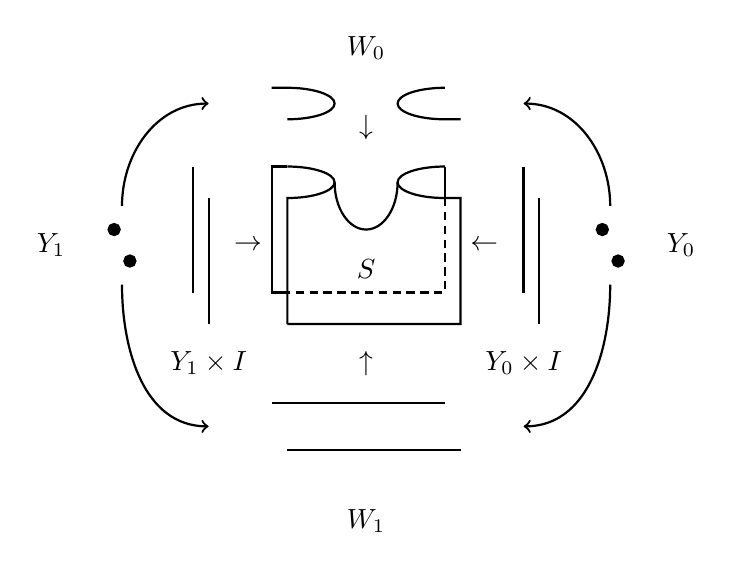
\begin{tikzpicture}[thick, scale = 2]
		% top
		\draw (1, 3.5) arc (90: 270: 0.3cm and 0.1cm) -- (1.1, 3.3) ;
		\draw (-.1, 3.5) -- (0,3.5) arc (90: -90: 0.3cm and 0.1cm);
		\node at (0.5, 3.75) {$W_0$};
		\node at (0.5, 3.25) {$\downarrow$};
		
		
		% main
		\draw (0, 3) arc (90: -90: 0.3cm and 0.1cm) -- (0, 2);
		\draw (1, 3) arc (90: 270: 0.3cm and 0.1cm) -- (1.1, 2.8) -- (1.1, 2) -- (0, 2);
		\draw (1,3) -- (1, 2.8); \draw [densely dashed] (1, 2.8) -- (1, 2.2) -- (0,2.2);
		\draw (.3, 2.9) arc (180: 360: 0.2cm and 0.3cm);
		\draw (0, 3) -- (-.1, 3) -- (-.1, 2.2) -- (0, 2.2);
		\node at (0.5, 2.35) {$S$};
		
		% bottom
		\draw (-0.1, 1.5) -- (1,1.5) (0,1.2) -- (1.1, 1.2);
		\node at (0.5, 0.75) {$W_1$};
		\node at (0.5, 1.75) {$\uparrow$};
		
		% left
		\draw (-0.5, 2.8) -- (-0.5, 2) (-0.6, 3) -- (-0.6, 2.2);
		\filldraw (-1, 2.4) circle (1pt) (-1.1, 2.6) circle (1pt); 
		\node at (-1.5, 2.5) {$Y_1$};
		\node at (-0.5,1.75) {$Y_1 \times I$};
		\node at (-0.25, 2.5) {$\rightarrow$};
		\draw [->] (-1.05, 2.75) to [out=90, in = 180] (-0.5, 3.4);
		\draw [->] (-1.05, 2.25) to [out=270, in = 180] (-0.5, 1.35);
		
		% right
		\draw (1.6, 2.8) -- (1.6, 2) (1.5, 3) -- (1.5, 2.2);
		\filldraw (2.1, 2.4) circle (1pt) (2, 2.6) circle (1pt); 
		\node at (2.5, 2.5) {$Y_0$};
		\node at (1.5,1.75) {$Y_0 \times I$};
		\node at (1.25, 2.5) {$\leftarrow$};
		\draw [->] (2.05, 2.75) to [out=90, in=0] (1.5,3.4);
		\draw [->] (2.05, 2.25) to [out=270, in=0] (1.5,1.35);
	\end{tikzpicture}
	

    \begin{figure}[ht]
	%\begin{center}
	 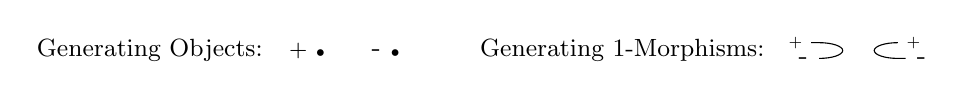
\begin{tikzpicture}

	\node at (-6, 1.5) {\small Generating Objects:};
	% objects:
	\node at (-4, 1.5) {\footnotesize + {\tiny $\bullet$}};
	\node at (-3, 1.5) {- {\tiny $\bullet$}};

	\node at (0, 1.5) {\small Generating 1-Morphisms:};
	% 1-morphisms
	\begin{scope}[xshift = 9cm, yshift = 2.1 cm]
	\draw (-6.6, -.5) -- (-6.5, -.5) arc (90: -90: 0.3cm and 0.1cm);
	\draw (-5.5, -.5) arc (90: 270: 0.3cm and 0.1cm) -- (-5.4, -.7);
	\node at (-6.8, -.5) {\tiny +};
	\node at (-6.7, -.7) {-};
	\node at (-5.3, -.5) {\tiny +};
	\node at (-5.2, -.7) {-};
	\end{scope}
	\end{tikzpicture}

	\begin{tikzpicture}

	\node at (-6, .5)   {\small Generating};
	\node at (-6, 0)   {\small 2-Morphisms:};

	\node at (-1,0) {
	$ \underbrace{
	 \begin{tikzpicture}
	% Draw the saddle, curve up
	\draw (0, 3) arc (90: -90: 0.3cm and 0.1cm) -- (0, 2);
	\draw (1, 3) arc (90: 270: 0.3cm and 0.1cm) -- (1.1, 2.8) -- (1.1, 2) -- (0, 2);
	\draw (1,3) -- (1, 2.8); \draw [densely dashed] (1, 2.8) -- (1, 2.2) -- (0,2.2);
	\draw (.3, 2.9) arc (180: 360: 0.2cm and 0.3cm);
	\draw (0, 3) -- (-.1, 3) -- (-.1, 2.2) -- (0, 2.2); 
	% Draw saddle, curve down
	\draw (2,2) arc (-90: 0: 0.3cm and 0.1cm);
	\draw [densely dashed] (2.3, 2.1) arc (0:90: 0.3cm and 0.1cm);
	\draw (2, 2.2) -- (1.9, 2.2) -- (1.9, 3) -- (3,3) -- (3, 2.8);
	\draw [densely dashed] (3, 2.8) -- (3, 2.2);
	\draw (2,2) -- (2, 2.8) -- (3.1, 2.8) -- (3.1, 2) -- (3,2);
	\draw (3,2) arc (270: 180: 0.3cm and 0.1cm);
	\draw [densely dashed] (3, 2.2) arc (90: 180: 0.3cm and 0.1cm); 
	\draw (2.3, 2.1) arc (180: 0: 0.2cm and 0.3cm);
	% Draw cap
	\begin{scope}[ xshift = 4cm]
	\draw (.1, 2) -- (0,2);
	\draw (0,2) arc (270: 180: 0.3cm and 0.1cm);
	\draw [densely dashed] (0, 2.2) arc (90: 180: 0.3cm and 0.1cm); 
	\draw [densely dashed] (.1, 2.2) -- (0, 2.2);
	\draw (.1,2) arc (-90: 0: 0.3cm and 0.1cm);
	\draw [dashed] (0.1, 2.2) arc (90:0: 0.3cm and 0.1cm);
	\draw (-.3, 2.1) arc (180: 0: 0.35cm and 0.4cm);
	\end{scope}
	%Draw cup
	\begin{scope}[ xshift = 5cm]
	\draw (.1, 3) arc (90: -90: 0.3cm and 0.1cm) -- (0, 2.8);
	\draw (0, 3) arc (90: 270: 0.3cm and 0.1cm) ;
	\draw (0, 3) -- (.1, 3);
	\draw (-.3, 2.9) arc (180: 360: 0.35cm and 0.4cm);
	\end{scope}
	\end{tikzpicture}
	}_\text{2D Morse generators}
	$};

	\node at (-2, -2) {
	$ \underbrace{
	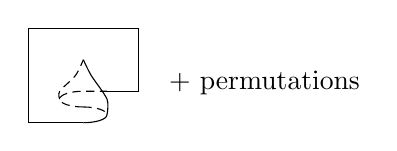
\begin{tikzpicture}
	\draw (0.5, 0) -- (-0.2,0) -- (-0.2, 1.2) -- (1.2, 1.2);
	\draw (0.5, 0) arc (-90: 0: 0.3cm and 0.1cm) ;
	\draw [densely dashed] (0.5, 0.2) arc (90: 0: 0.3cm and 0.1cm) ;
	\draw [densely dashed] (0.5, 0.2) arc (270: 90: 0.3cm and 0.1cm) -- (0.8, 0.4);
	\draw (0.8, 0.4) -- (1.2, 0.4) -- (1.2, 1.2);
	\node (C) at (0.5, 0.8) {};
	%\draw (0.8, 0.1) -- (C.center);
	%\draw [dashed] (0.2, 0.3) -- (C.center);
	\draw  plot [smooth] coordinates{(0.8,0.1) (0.8,0.3) (0.6, 0.6) (C.center)}; 
	\draw [densely dashed] plot [smooth] coordinates{(0.2,0.3) (0.2,0.4) (0.4, 0.6) (C.center)}; 
	\node at (2.8, 0.5) { + permutations};
	\end{tikzpicture}
	}_\text{Cusp generators}$
	};


	\node at (-6, -4.0) {\small Relations among};
	\node at (-6, -4.5) {\small 2-Morphisms:};


	%Morse

	\node at (-5.5, -6.2) {
	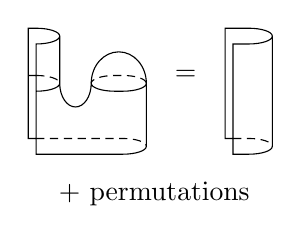
\begin{tikzpicture}
	% Morse relation
	\begin{scope} []
	\draw (0.1, 0.2) -- (0, 0.2) -- (0, 1.6) -- (0.1, 1.6) arc (90: -90: 0.3cm and 0.1cm) -- 
		(0.1, 0) -- (1.2, 0) arc (-90: 0: 0.3cm and 0.1cm) -- (1.5, 0.9)
		arc (0: 180: 0.35cm and 0.4cm) arc (360: 180: 0.2cm and 0.3 cm) -- (0.4, 1.5)
		(1.5, 0.9) arc (0: -90: 0.3cm and 0.1cm) -- (1.1, 0.8) arc (270: 180: 0.3cm and 0.1cm)
		(0,1) -- (0.1,1) (0.1, 0.8) arc (-90: 0: 0.3cm and 0.1cm);
	\draw [densely dashed] (0.1, 1) arc (90: 0: 0.3cm and 0.1cm) (1.5, 0.9) arc (0: 90: 0.3cm and 0.1cm) -- 
		(1.1, 1) arc (90: 180: 0.3cm and 0.1cm) (0.1, 0.2) -- (1.2, 0.2) arc (90: 0: 0.3cm and 0.1cm);
	\end{scope}
	\begin{scope}[xshift = 2cm, yshift = 1cm]
	 \node at (0,0) {=};
	\end{scope}
	% Morse identity
	\begin{scope}[xshift = 2.5cm,]
	\draw (.1,.2) -- (0, 0.2) --(0,1.6) -- (.3, 1.6) arc (90: -90:  0.3cm and 0.1cm) -- (0.1, 1.4) 
		-- (0.1,0) -- (.3, 0) arc (-90: 0:  0.3cm and 0.1cm)  -- (.6, 1.5);
	\draw [densely dashed] (.1, .2) -- (.3, .2) arc (90: 0: 0.3cm and 0.1cm);
	\end{scope}
	\begin{scope}[xshift = 1.6cm,  yshift = -.5cm]
	\node at (0,0) {+ permutations};
	\end{scope}
	\end{tikzpicture}
	};


	%swallowtail
	\node at (-0.5, -5.5) {=};
	\node at (-1, -5.8) {
	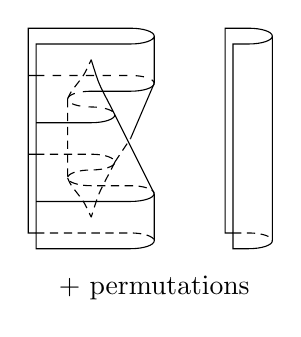
\begin{tikzpicture}
	\begin{scope}[]
	% outside framing, top and bottom
	\draw (.1,.2) -- (0, 0.2) --(0,2.8) -- (1.3,2.8) arc (90: -90:  0.3cm and 0.1cm) -- (0.1, 2.6) 
		-- (0.1,0) -- (1.3, 0) arc (-90: 0:  0.3cm and 0.1cm) -- (1.6, 0.7) (1.6, 2.7) -- (1.6, 2.1);
	\draw [densely dashed] (0.1,0.2) -- (1.3, 0.2) arc (90: 0:  0.3cm and 0.1cm);
	%middle top
	\draw (0, 2.2) -- (0.1, 2.2) (.8, 2) -- (1.3, 2) arc (-90: 0:  0.3cm and 0.1cm) 
		(0.1, 1.6) -- (0.8, 1.6) arc (-90: 0:  0.3cm and 0.1cm);
	\draw [dashed] (0.1, 2.2) -- (1.3, 2.2) arc (90: 0:  0.3cm and 0.1cm) 
		(.8, 2) arc (90: 270:  0.3cm and 0.1cm) arc (90: 0:  0.3cm and 0.1cm);
	% middle bottom and center
	\draw (0, 1.2) -- (0.1, 1.2) (0.1, 0.6) -- (1.3, 0.6) arc (-90: 0:  0.3cm and 0.1cm);
	\draw [densely dashed] (0.1, 1.2) -- (0.8, 1.2) arc (90: -90:  0.3cm and 0.1cm) 
		arc (90: 270:  0.3cm and 0.1cm) -- (1.3, 0.8) arc (90: 0:  0.3cm and 0.1cm);
	\draw [densely dashed] (.5, 1.9) -- (.5, 0.9) plot [smooth] coordinates{(.5,1.9) (.55, 2) (.7, 2.2)  (.8,2.4)}
		plot [smooth] coordinates{(.5,0.9) (.55, .8) (.7, 0.6)  (.8,0.4)}
		plot [smooth] coordinates{ (1.1,1.1) (1.05, 1) (.9, 0.7)  (.8,0.4)}
		(1.1, 1.1) -- (1.3, 1.4) ;
	\draw plot [smooth] coordinates{(1.1, 1.7)  (1.05, 1.8) (.9, 2.1)  (0.8, 2.4)}
		(1.1, 1.7) -- (1.6, 0.7) (1.3, 1.4) -- (1.6, 2.1);
	\end{scope}
	% swallowtial identity
	\begin{scope}[xshift = 2.5cm]
	\draw (.1,.2) -- (0, 0.2) --(0,2.8) -- (.3,2.8) arc (90: -90:  0.3cm and 0.1cm) -- (0.1, 2.6) 
		-- (0.1,0) -- (.3, 0) arc (-90: 0:  0.3cm and 0.1cm)  -- (.6, 2.7);
	\draw [densely dashed] (.1, .2) -- (.3, .2) arc (90: 0: 0.3cm and 0.1cm);
	\end{scope}
	\begin{scope}[xshift = 1.6cm,  yshift = -.5cm]
	\node at (0,0) {+ permutations};
	\end{scope}
	\end{tikzpicture}
	};



	% Flip
	\node at (-5, -9.7) {
	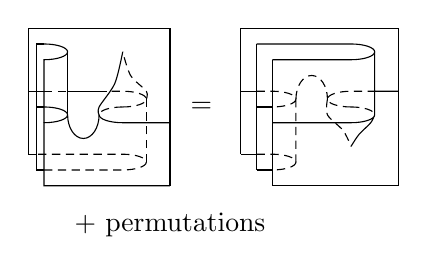
\begin{tikzpicture}
	% Part of the flip relation. 
	\begin{scope}[yshift = -2cm]
	\draw (0, 3) arc (90: -90: 0.3cm and 0.1cm) -- (0, 2) -- (1.6,2); %too long
	\draw [densely dashed] (1,3) arc (-90: 90: 0.3cm and 0.1cm) -- (0.8, 3.2); 
	\draw [densely dashed] (1,3) arc (90: 180: 0.3cm and 0.1cm); 
	\draw (0.7, 2.9) arc (180: 270: 0.3cm and 0.1cm) -- (1.6, 2.8) ;
	%\draw (1,3) -- (1, 2.8); 
	\draw [densely dashed] (0, 2.2) -- (1,2.2) arc (-90: 90: 0.3cm and 0.1cm) -- (-.1, 2.4);
	\draw [densely dashed] (1.3, 2.3) -- (1.3, 3.1);
	\draw (.3, 2.9) arc (180: 360: 0.2cm and 0.3cm);
	\draw (0, 3) -- (-.1, 3) -- (-.1, 2.2) -- (0, 2.2); 
	\node (C) at (1, 3.7) {};
	\draw plot [smooth] coordinates{(0.7, 2.9) (0.7,3) (0.9, 3.3) (C.center)}; 
	\draw [densely dashed] plot [smooth] coordinates{(1.3, 3.1) (1.3,3.2) (1.1, 3.4) (C.center)}; 
	\draw (-.1, 2.4) -- (-.2, 2.4) -- (-.2, 3.2) -- (0, 3.2);
	\draw [densely dashed] (0, 3.2) -- (.3, 3.2);
	\draw (.3, 3.2) -- (0.8, 3.2);
	\draw (-.2, 3.2) -- (-.2, 4) -- (1.6,4) -- (1.6, 2);
	\draw (0, 3.8) arc (90: -90: 0.3cm and 0.1cm) -- (0, 2.8);
	\draw (0, 3.8) -- (-.1, 3.8) -- (-.1, 3); 
	\draw (.3, 3.7) -- (.3, 2.9);
	\end{scope}
	\begin{scope}[xshift = 2cm, yshift=1cm]
	\node at (0,0) {=};
	\end{scope}
	% Other part of the flip relation
	\begin{scope}[xshift = 2.5cm,]
	%perimeter
	\draw (0,0.4) -- (0,2) -- (2, 2) -- (2, 0) -- (0.4, 0) -- (0.4, 1.6);
	\draw (0.2, 0.2) -- (0.2, 1.8);
	%top
	\draw (0.2, 1.8) -- (1.4, 1.8) arc (90: -90:  0.3cm and 0.1cm) -- (0.4, 1.6);
	%bottom
	\draw (0, 0.4) -- (0.2, 0.4) (0.2, 0.2) -- (0.4, 0.2);
	\draw [densely dashed] (0.2, 0.4) -- (0.4, 0.4) arc (90: -90:  0.3cm and 0.1cm);
	%left middle
	\draw (0, 1.2) -- (0.2, 1.2) (0.2, 1) -- (0.4, 1);
	\draw [densely dashed] (0.2, 1.2) -- (0.4, 1.2) arc (90: -90:  0.3cm and 0.1cm) (0.7, 1.1) -- (0.7, 0.3);
	%right middle
	\draw (0.4, 0.8) -- (1.4, 0.8) arc (-90: 0: 0.3cm and 0.1cm) -- (1.7, 1.7) 
	(1.7, 1.2) -- (2, 1.2) plot [smooth] coordinates{ (1.7, 0.9) (1.65, 0.8) (1.5, 0.65)  (1.4, 0.5)}; 
	\draw [densely dashed] (1.4, 1) arc (90: 0: 0.3cm and 0.1cm) (1.4, 1) arc (270: 90: 0.3cm and 0.1cm) 
	-- (1.7, 1.2) (0.7, 1.1) arc (180: 0: 0.2cm and 0.3cm )
	plot [smooth] coordinates{(1.1,1.1) (1.1, 0.9) (1.3, 0.7) (1.4, 0.5)};
	\end{scope}
	\begin{scope}[xshift = 1.6cm,  yshift = -.5cm]
	\node at (0,0) {+ permutations};
	\end{scope}
	\end{tikzpicture}
	};


	%%% Cusp Inversion AI
	\begin{scope}[xshift = -1cm, yshift = -9.5cm]
	\draw (0.5, 1.2) -- (-0.2,1.2) -- (-0.2,-0.5) -- (0.2, -0.5);
	\draw (0.5, 1.2) arc (90: -90: 0.3cm and 0.1cm) arc (90: 270: 0.3cm and 0.1cm) -- (0.8, 0.8);
	\draw [densely dashed] (0.2, -0.5) -- (0.5,-0.5) arc (90: -90: 0.3cm and 0.1cm) arc (90: 180: 0.3cm and 0.1cm);
	\draw (0.2, -0.8) arc (180: 270: 0.3cm and 0.1cm) -- (0.8, -0.9);
	\draw (0.8, 0.8) -- (1.2, 0.8) -- (1.2, -0.9) -- (0.8, -0.9);
	\node (C) at (0.5, 0.4) {}; 
	\node (D) at (0.5, -0.1) {};
	\draw  plot [smooth] coordinates{(0.8,1.1) (0.8,0.9)}; 
	\draw [densely dashed] plot [smooth] coordinates{ (0.8,0.9) (0.6, 0.6) (C.center)}; 
	\draw  plot [smooth] coordinates{(0.2,0.9) (0.2,0.8) (0.4, 0.6) (C.center)}; 
	\draw  plot [smooth] coordinates{(0.2,-0.8) (0.2,-0.6) (0.4, -0.4) (D.center)}; 
	\draw [densely dashed] plot [smooth] coordinates{(0.8,-0.6) (0.8,-0.5) (0.6, -0.3) (D.center)}; 
	\end{scope}

	%%% Cusp Inversion AII
	\begin{scope}[xshift = 2cm, yshift = -9.5cm]
	\draw (0.5, 1.2) -- (-0.2,1.2) -- (-0.2,-0.5) -- (0.2, -0.5); %(0.5, -0.5) ;
	\draw (0.5, 1.2) arc (90: -90: 0.3cm and 0.1cm) arc (90: 270: 0.3cm and 0.1cm) -- (0.8, 0.8);
	\draw [densely dashed] (0.2, -0.5) -- (0.5,-0.5) arc (90: -90: 0.3cm and 0.1cm) arc (90: 180: 0.3cm and 0.1cm);
	\draw (0.2, -0.8) arc (180: 270: 0.3cm and 0.1cm) -- (0.8, -0.9);
	\draw (0.8, 0.8) -- (1.2, 0.8) -- (1.2, -0.9) -- (0.8, -0.9);
	\node (C) at (0.5, 0.4) {};
	\draw (0.2, 0.9) -- (0.2, -0.8) (0.8, 1.1) -- (0.8, -0.6);
	\end{scope}

	\node at (1, -9.5) {=};
	\node at (1, -12) {=};


	%%% Cusp Inversion BI
	\begin{scope}[xshift = -1cm, yshift = -11.2cm]
	\draw (1.2, 0.4) -- (-0.2,0.4) -- (-0.2,-0.5) -- (0.2, -0.5);
	\draw [densely dashed] (0.2, -0.5) -- (0.5,-0.5) arc (90: -90: 0.3cm and 0.1cm) arc (90: 180: 0.3cm and 0.1cm);
	\draw (0.2, -0.8) arc (180: 270: 0.3cm and 0.1cm) -- (0.8, -0.9);
	\draw  (1.2, 0.4) -- (1.2, -0.9) -- (0.8, -0.9);
	\draw (1.2, -0.9) -- (1.2, -1.6) -- (-0.2, -1.6) -- (-0.2, -0.5); 
	\node (D) at (0.5, -0.1) {};
	\draw  plot [smooth] coordinates{(0.2,-0.8) (0.2,-0.6) (0.4, -0.4) (D.center)}; 
	\draw [densely dashed] plot [smooth] coordinates{(0.8,-0.6) (0.8,-0.5) (0.6, -0.3) (D.center)}; 
	\node (C) at (0.5, -1.3) {}; 
	\draw  plot [smooth] coordinates{(0.8,-0.6) (0.8,-0.7)}; 
	\draw [densely dashed] plot [smooth] coordinates{ (0.8,-0.7) (0.6, -1) (C.center)}; 
	\draw  plot [smooth] coordinates{(0.2,-0.8) (0.2,-0.9) (0.4, 0.-1.1) (C.center)}; 
	\end{scope}

	%%% Cusp Inversion BII
	\begin{scope}[xshift = 2cm, yshift = -12cm]
	% 
	\draw  (0.8, 0.8) to [out = 180, in = 0] (0.2, 1.2) -- (-0.2,1.2) -- (-0.2,-0.5) -- (0.2, -0.5) to [out = 0, in = 180] (0.8, -0.9);
	%\draw (0.5, 1.2) arc (90: -90: 0.3cm and 0.1cm) arc (90: 270: 0.3cm and 0.1cm) -- (0.8, 0.8);
	%\draw [densely dashed] (0.2, -0.5) -- (0.5,-0.5) arc (90: -90: 0.3cm and 0.1cm) arc (90: 180: 0.3cm and 0.1cm);
	%\draw (0.2, -0.8) arc (180: 270: 0.3cm and 0.1cm) -- (0.8, -0.9);
	\draw (0.8, 0.8) -- (1.2, 0.8) -- (1.2, -0.9) -- (0.8, -0.9);

	\end{scope}


	%\end{scope}

	 \end{tikzpicture}
	%\end{center}
	\caption{Oriented Generators and Relations}
	\label{fig:OrientedGenAndRel}	
\end{figure}